% Beamer template
% Author: Ozgur Taylan TURAN
% Delft University of Technology

\documentclass[aspectratio=169]{beamer}
% PACKAGES
\usepackage[english]{babel}
\usepackage{graphicx}
\usepackage{animate}
%\usepackage{calc}
\usepackage{calligra}
\usepackage[absolute,overlay]{textpos}
\usepackage[T1]{fontenc}
%\usefonttheme{serif}
\usefonttheme{professionalfonts}
\usepackage{amsmath}
\usepackage{palatino}
\usepackage{mathpazo}
\usepackage{graphicx}
\graphicspath{{Figures/}}
%\usepackage{subfig}
\usepackage{tikz}
\usetikzlibrary{shapes,arrows}
\usepackage{xcolor}
\usepackage[T1]{fontenc}
%\usefonttheme{serif}
%\usepackage{titling}
\usepackage{graphicx}
%\usepackage{subfig}
%\usepackage{tikz}
%\usetikzlibrary{shapes,arrows}
\usepackage{mathtools}
\usepackage{cancel}
% CUSTOM PACKAGES
\usepackage{/home/taylanot/texmf/tex/beamerthemetot}
\input{/home/taylanot/texmf/presentation/tune.tex}

 % COVER PAGE INFO   
\newcommand{\mytitle}{\color{White}\huge{\textbf{PINNs \#3}}}
\newcommand{\mysubtitle}{\color{Pink}\Large{\textbf{Physics-Informed Kernel Regression}}}
\newcommand{\myauthor}{\color{White}\textcalligra{\LARGE Ozgur Taylan Turan}}
\newcommand{\authorlabel}{\small O.T. Turan}
\author{\authorlabel}


\begin{document}
% COVER PAGE

{
\def\beamer@entrycode{\vspace*{-\headheight}}
\setbeamertemplate{frametitle}[default][center]
\setbeamertemplate{navigation symbols}{}
\usebackgroundtemplate{
\includegraphics[width=\paperwidth,height=\paperheight]{cover/coverart.pdf}}

\begin{frame}[plain] 

\begin{minipage}{\textwidth}
	\centering{\mytitle} \\
	%\vspace{1cm}
	%\centering{\mysubtitle} \\
	\vspace{1cm}
	\centering{\color{White}November 15, 2021} \\
	\vspace{1cm}
	\centering{\myauthor}\\
\end{minipage}
\end{frame}
}


\begin{frame}
	\centering
	\mysubtitle
\end{frame}

\section{Past Meeting}
\begin{frame}{Past}
  \centering
  Whole report is coming with the results of non-linear observations as well!
\end{frame}

\section{PINN}
\begin{frame}{Physics-Informed Neural Networks}
  \centering
  \begin{itemize}
    \item Side-project after David's Coffee-talk
  \end{itemize}
  \color{Pink} Main Idea:\color{Black}
  \begin{itemize}
    \item Solve $ODE:y^{\prime\prime}=-1$ with BCs $y(-1)=0$ and $y(1)=0$, where $y(x)$ and $y^\prime=\frac{dy}{dx}$
    \item Assume your solution $y(x)$ is given by a function $\mathcal{M}(x,\mathbf{w})$,
    \item Then,solution can be obtained by minimizing $\mathcal{L}_{\text{total}}:=\mathcal{L}_{\text{domain}}+\mathcal{L}_{\text{boundary}}$
    \item $\mathcal{L}_{\text{domain}}:=MSE(\mathcal{M}^{\prime\prime}(x)-1)$
    \item $\mathcal{L}_{\text{bc}}:=MSE(\mathcal{M}(-1)+\mathcal{M}(+1))$
  \end{itemize}
\end{frame}

\begin{frame}{It works!}
  \begin{itemize}
    \item Works beautifully if you sample enough points (x)
    \item But, why just neural networks, we can put any model there?
  \end{itemize}
\end{frame}

\begin{frame}{Let's look at the kernelized Linear Regression}
  \centering
  \begin{minipage}{0.3\textwidth}
    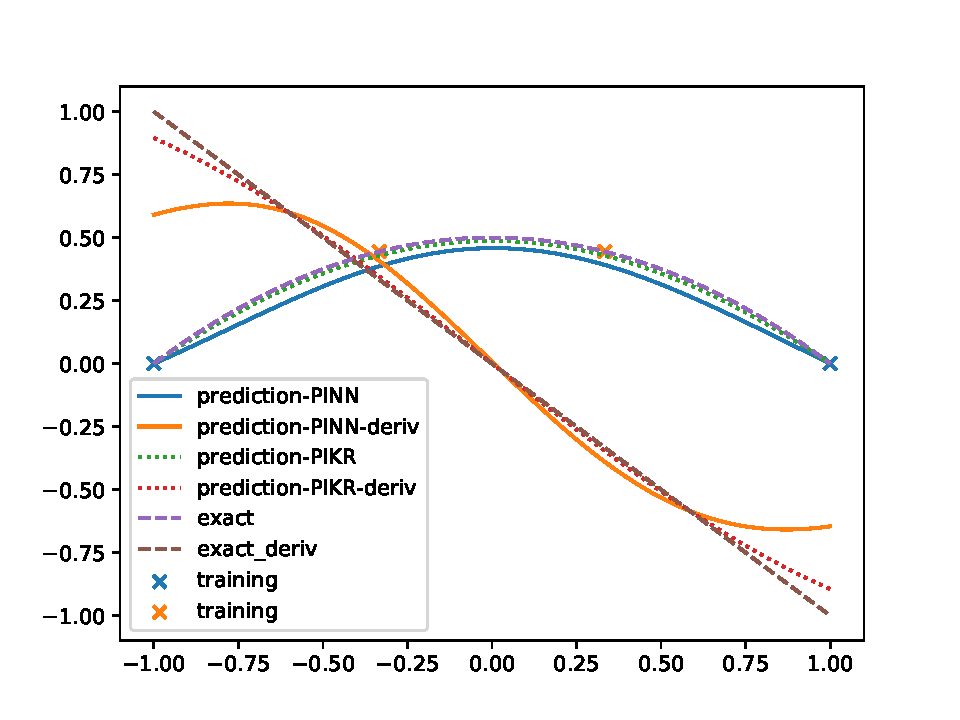
\includegraphics[width=\textwidth]{pinn-4.pdf}
  \end{minipage}%
  \begin{minipage}{0.3\textwidth}
    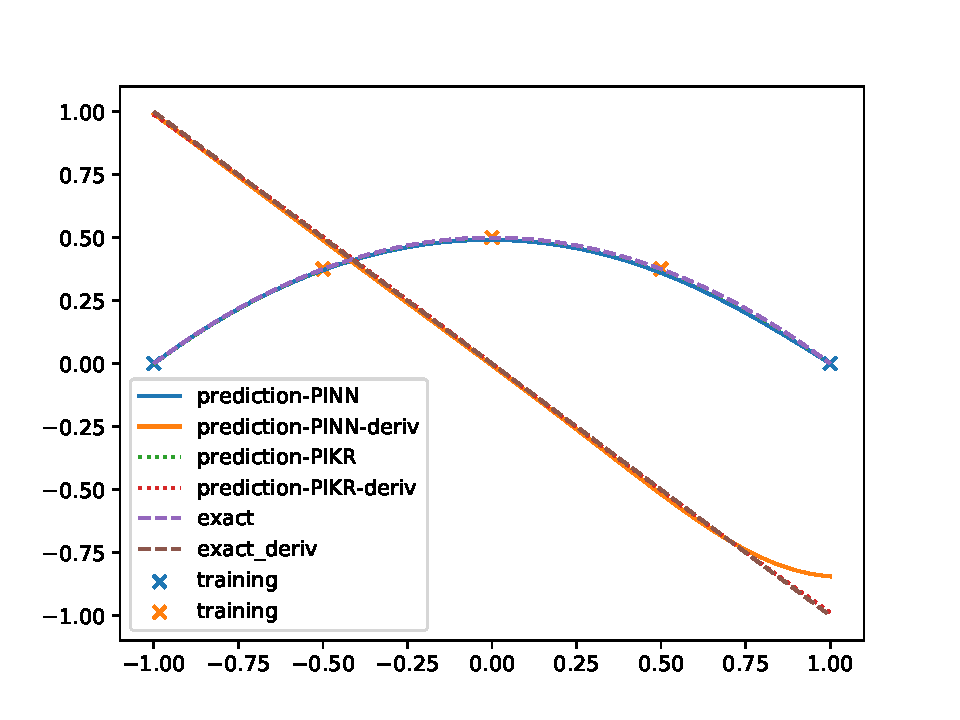
\includegraphics[width=\textwidth]{pinn-5.pdf}
  \end{minipage}%
  \begin{minipage}{0.3\textwidth}
    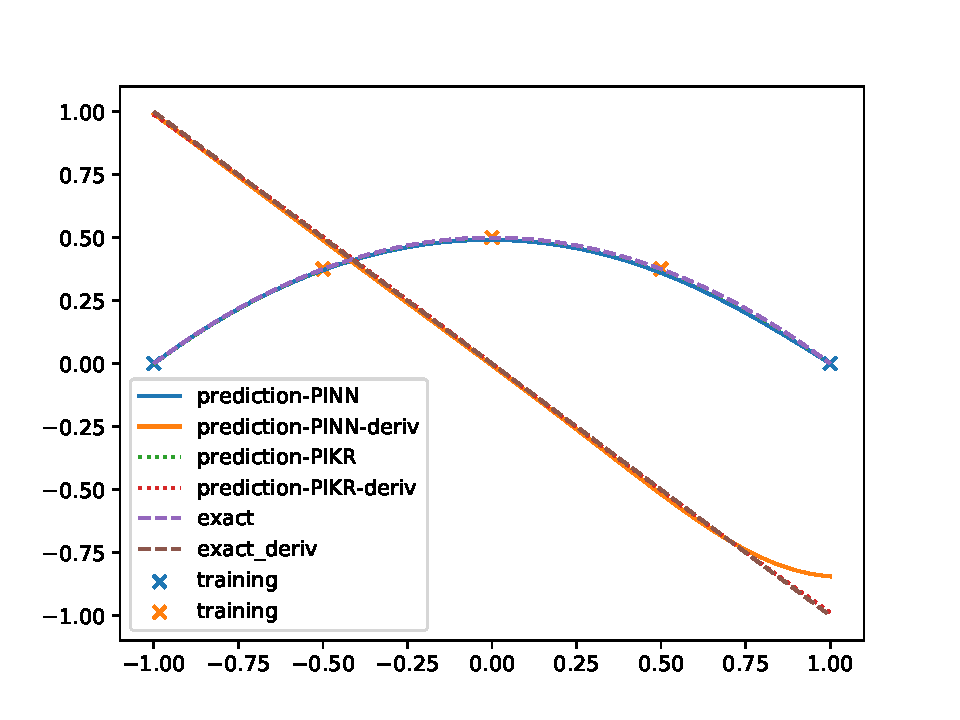
\includegraphics[width=\textwidth]{pinn-5.pdf}
  \end{minipage}
  \begin{itemize}
    \item If you don't sample enough data you do not simply satisfy the equation at given points although you have the flexibility!
    \item Is it a bad idea to use the same loss minimization for determining kernel parameters?
    \item Shallow and a wide network 2 hidden layers and 100 neurons/layer
  \end{itemize}
\end{frame}

\begin{frame}{Why not use kernel methods not considered?}
  \centering
    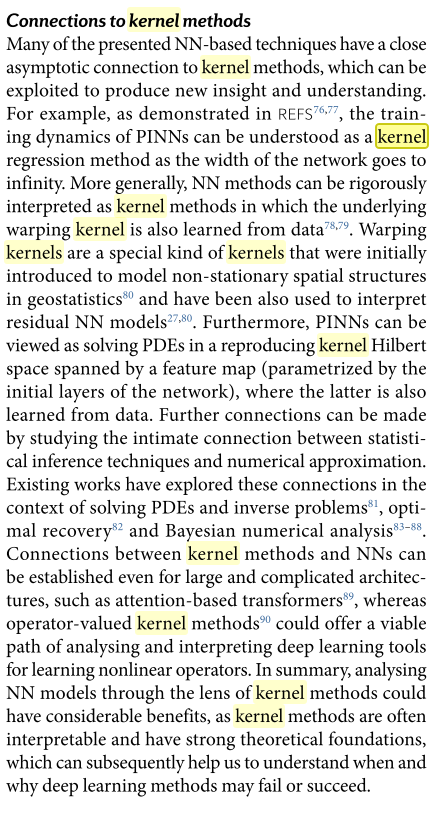
\includegraphics[width=0.3\textwidth]{kernel.png}
    \begin{itemize}
      \item Kernels are only considered for explaining and understanding neural networks?
    \end{itemize}
\end{frame}


\section{Extra}
\begin{frame}{Polynomial regression}
  \centering
    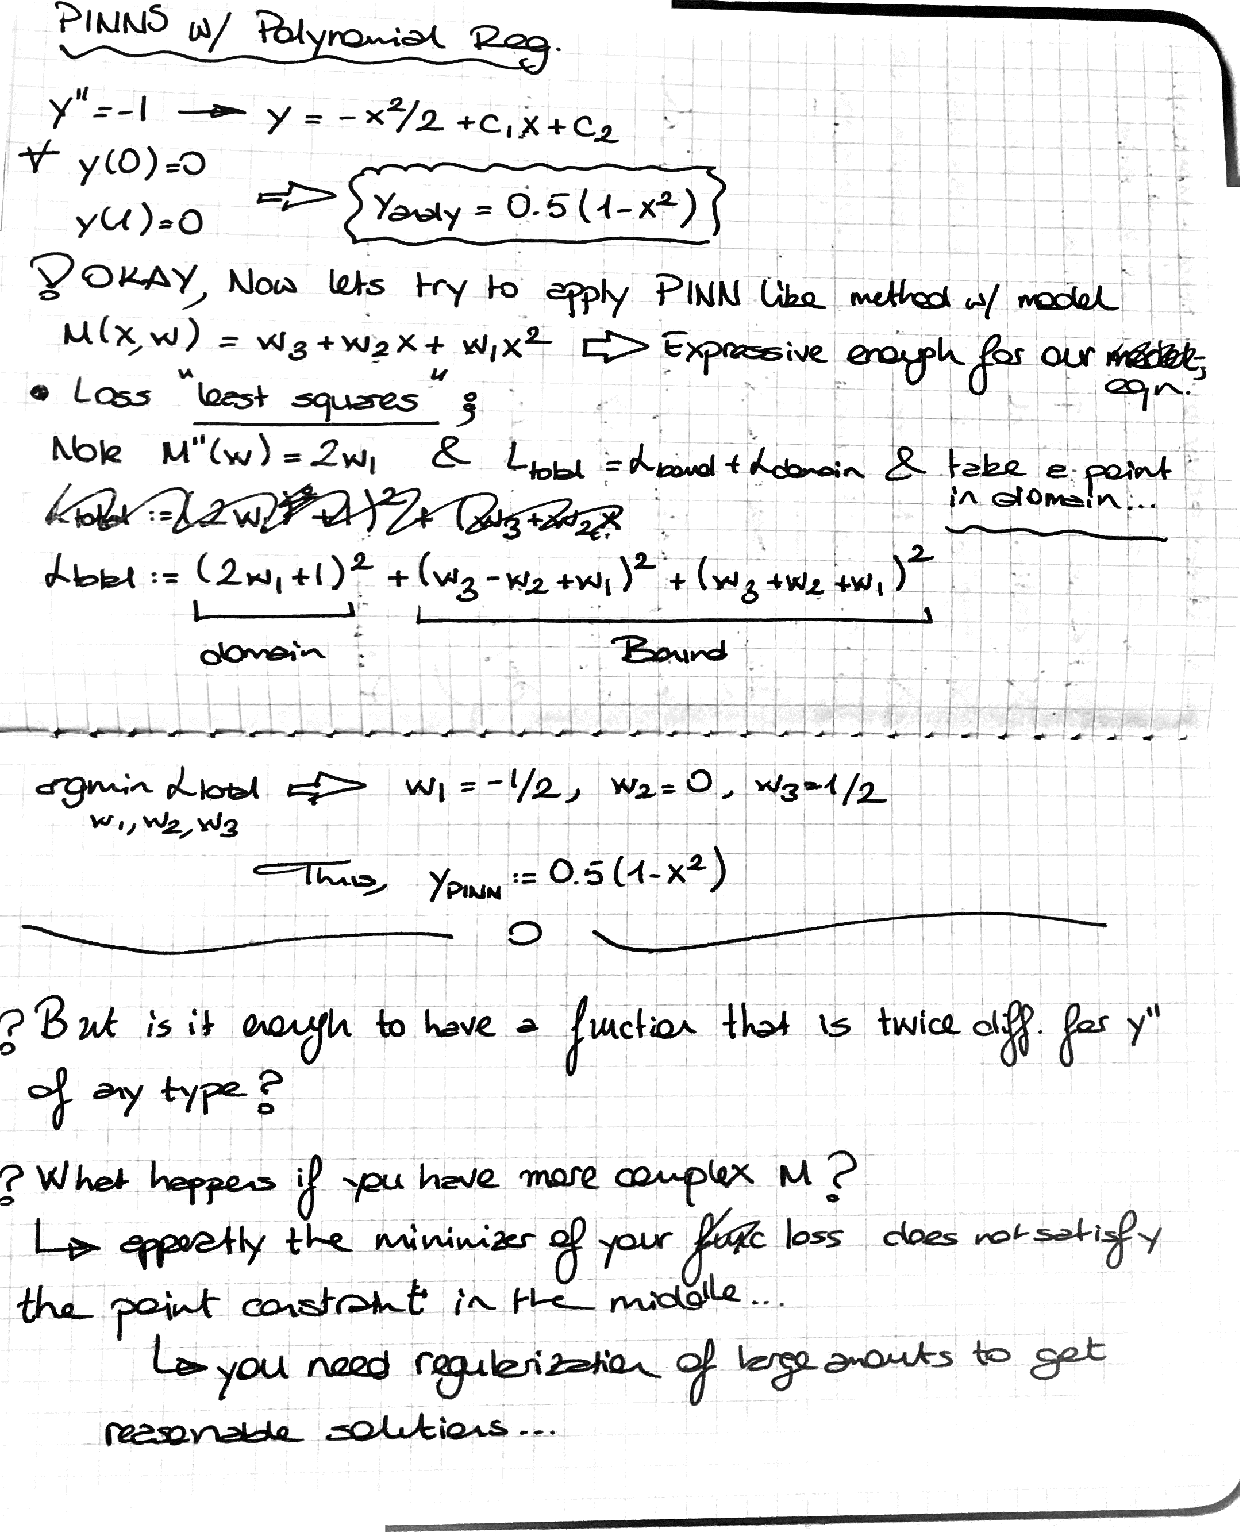
\includegraphics[width=0.3\textwidth]{pinnpoly.pdf}
\end{frame}

\begin{frame}{Polynomial regression, increase model complexity!}
  \centering
    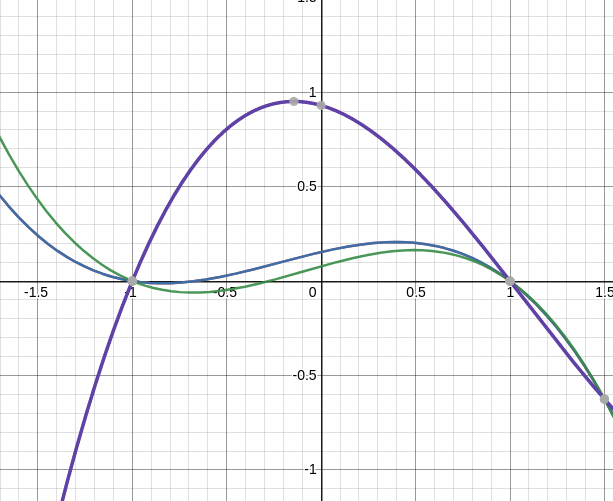
\includegraphics[width=0.3\textwidth]{models.png}
\end{frame}

\begin{frame}{Regularize the loss from the domain!}
  \centering
    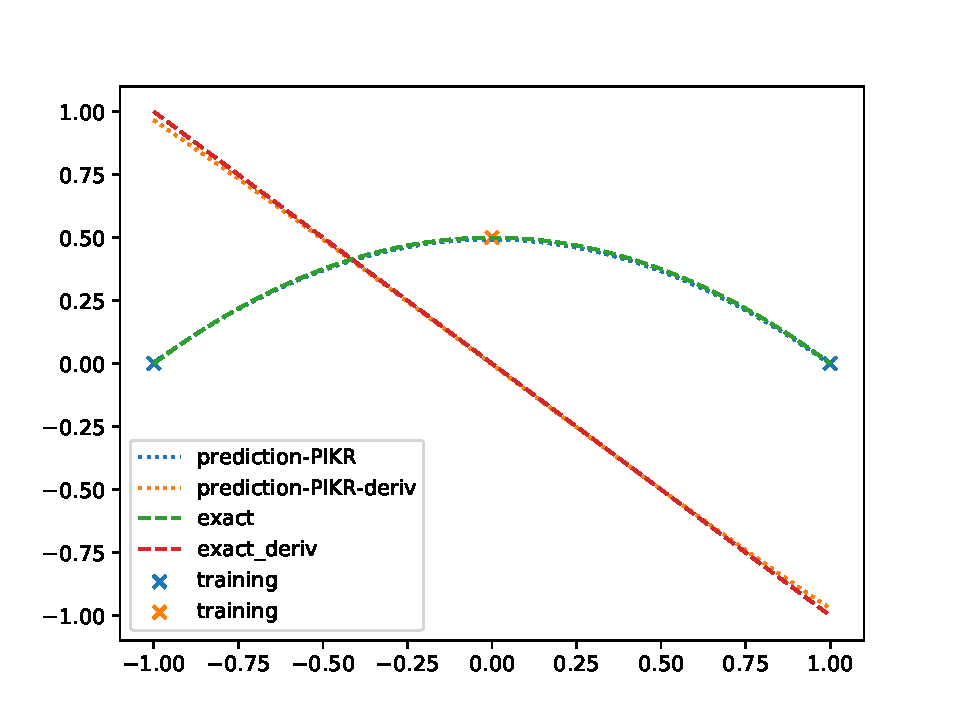
\includegraphics[width=0.3\textwidth]{pinn-3.pdf}
\end{frame}

\begin{frame}{Conclusion}
  \centering
  \begin{itemize}
    \item Either use enough data for your models needs.
    \item We do not need to use NN's for ODE solutions other methods are also viable and some can even give exact solutions if you know the nature of your problem. But, that is not always the case, so use of complex models are justifiable???
    \item I believe PINNs should be investigated with the help of kernel methods definitely more, as they might be more capable then we think!
  \end{itemize}
\end{frame}







\end{document}
